% !TEX root = ../Thesis.tex
\chapter{DESIGN AND IMPLEMENTATION}
\section{Web application architecture}
The initial application is a client-side React application built with Vite. Lesson content is stored in a JavaScript data module. The user selects a lesson, answers its question, and receives answer feedback. React state tracks selections while the browser session remains active.

\begin{figure}[htbp]
\centering
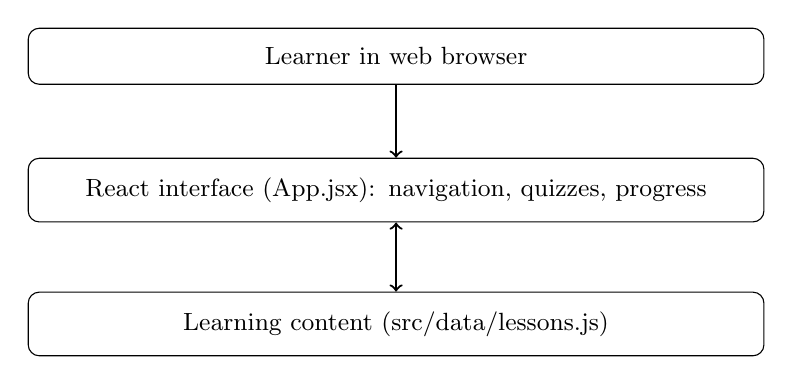
\begin{tikzpicture}[node distance=12mm, every node/.style={font=\small}]
  \tikzstyle{block}=[draw, rounded corners, text width=0.73\textwidth, align=center, inner sep=7pt]
  \node[block] (browser) {Learner in web browser};
  \node[block, below of=browser, node distance=17mm] (react) {React interface (App.jsx): navigation, quizzes, progress};
  \node[block, below of=react, node distance=17mm] (data) {Learning content (src/data/lessons.js)};
  \draw[->, thick] (browser) -- (react);
  \draw[<->, thick] (react) -- (data);
\end{tikzpicture}
\caption{Simplified architecture of the initial OLT prototype.}
\label{fig:architecture}
\end{figure}

\section{Learning modules}
Three initial learning topics are included: understanding stormwater, sustainable drainage, and flood resilience. The content and quiz items are introductory examples that can be revised after subject-matter review.

\section{User interface and responsiveness}
The interface uses a responsive layout, readable typography, and native form controls. It includes an explicit navigation region for learning modules, a progress indicator, radio-button answers, and status feedback.

\section{Accessibility implementation}
The initial source includes a skip link, fieldset and legend for each question, explicit radio labels, visible focus styles, and a status region for quiz feedback. These features provide a foundation for accessibility; keyboard tests, screen-reader tests, contrast checks, and responsive tests remain necessary.

\section{Known prototype limitations}
Learner answers are held in component state and are not saved to a database or browser storage. The current progress indicator reflects answered knowledge checks, not verified completion or mastery. There is no authentication or administrative backend in this prototype.
